\documentclass[16pt, margin=16pt]{standalone}
\usepackage{tikz}
\usetikzlibrary{arrows}
% \usetikzlibrary{decorations.pathreplacing}
% \tikzset{>=stealth'}

\tikzset{grid/.style = {
    step = .5cm, 
    lightgray, 
    very thin
}}

\begin{document}
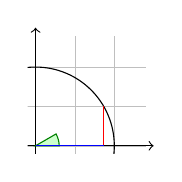
\begin{tikzpicture}
    \clip 
        (-0.1, -0.1) rectangle (1.5, 1.5)
    ;
    
    % Grid
    \draw [grid] (-1.4, -1.4) grid (1.4, 1.4);
    
    % Lines
    \draw 
        [->] (-1.5, 0) -- (1.5, 0)
    ;
    \draw
        [->] (0, -1.5) -- (0, 1.5)
    ;

    \draw 
        (0, 0) circle (1cm)
    ;
    \filldraw 
        [fill = green!20!white, draw = green!50!black]
        (0, 0) 
        -- (0.3, 0) 
        arc [start angle = 0, end angle = 30, radius = 0.3] 
        -- cycle
    ;
    \draw
        [red] 
        (30:1) -- +(0, -0.5)
    ;
    \draw
        [blue]
        (30:1) ++(0, -0.5) -- (0, 0)
    ;

\end{tikzpicture}
\end{document}